\documentclass[a4paper,10pt]{report}
\usepackage[utf8]{inputenc}
\usepackage{multirow}
\usepackage{graphicx}
\usepackage[margin=1.0in]{geometry}


% Title Page
\title{Compositing Optimizations in VisIt for Insitu Visualization}
\author{Burlen Loring and Oliver Ruebel}


\begin{document}
\maketitle

\begin{abstract}
\end{abstract}

\section{Introduction}



I have some results to report from our rendering infrastructure work that was done in conjunction with our recent insitu paper. Described below. Just wanted to let you know more about the work and the results we got. It could be claimed under sdav or 1401043 and I want to put it in an lbl tech report.

I have a patch for visit that enables ordered compositing and depth peeling in parallel. While my intention was to just enable order compositing, I was also able to address a number of performance issues, and optimize some key sections of code. The result is overall faster rendering and compositing in VisIt.





\section{Optimizations}
About the optimizations
The main optimization is ordered compositing. However, I ended up replacing VisIt's compositers with a new one I call the ProgrammableCompositer. A few key aspects are that the kernels are vectoirized by the compiler at -O3, it uses threads to overlap compositing and data transfer (streaming), and it could be programmed with different communication pattern.

There were a number of other optimization that I made to address obvious performance issues. These included, vectorizing some key sections of code, eliminating memcpy when you could pass a pointer, eleiminate unnecessary readback from gpu, reducing and eliminating communications, skip executing vtk pipeline when it's not needed, and so on. For the most part addressing efficiency issues.

I will write a white paper about this stuff.

\subsection{Ordered Compositing}
\begin{figure}
 \centering
 \begin{minipage}{0.48\textwidth}
 \begin{center}
 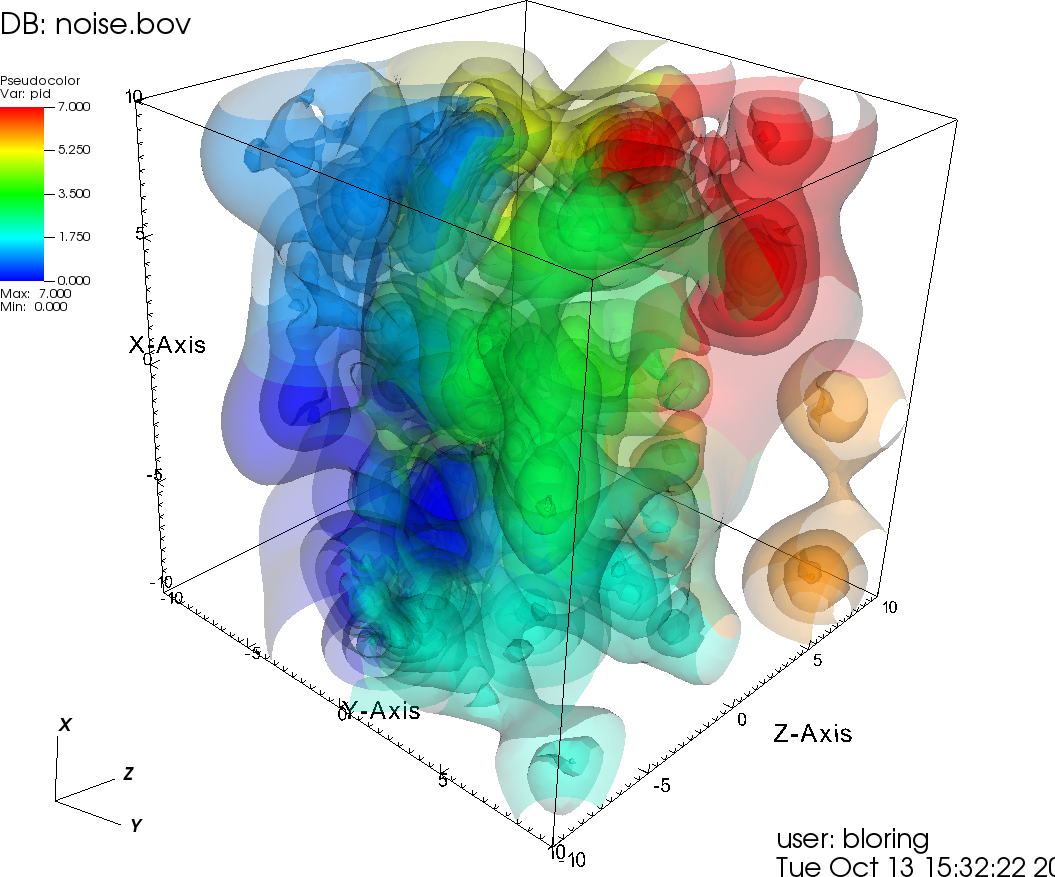
\includegraphics[height=2.5in]{./order_composite_example_color.png}
\end{center}

  \end{minipage}
  \begin{minipage}{0.48\textwidth}
\begin{center}
 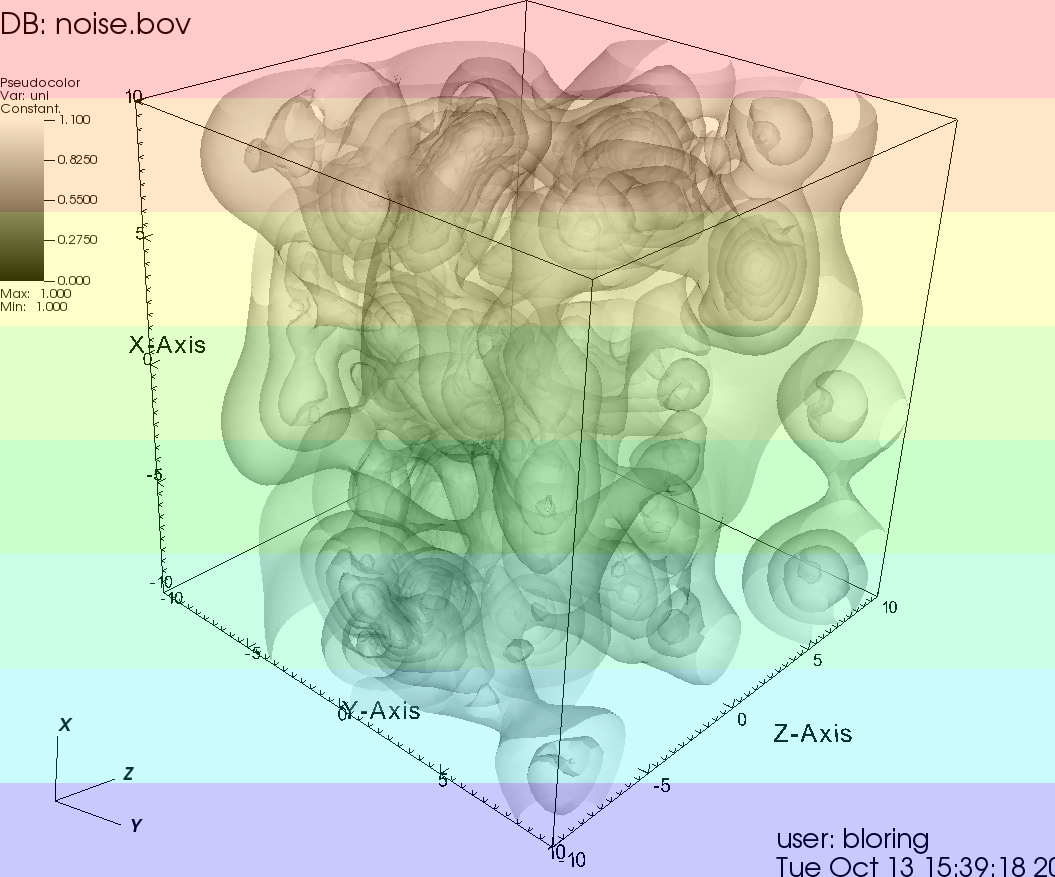
\includegraphics[height=2.5in]{./tiled_image_example_color.png}
\end{center}
  \end{minipage}
 \caption{Order compositing and image tiled compositing examples. This test dataset is distributed over 8 cores and then 10 iso-surfaces are computed. The original data decomposition is shown on the left. Ordered compositing renders the data using this decomposition. The tiled image compositing decomposition is shown on the right. Image tiled compositing transfers the data from the original decomposition(left) onto the new decomposition(right) during rendering.}
 \label{fig:vpic_data}
\end{figure}



order = 4 5 6 0 7 1 2 3 
round 0:
4 <- 5 6 <- 0 7 <- 1 2 <- 3 
round 1:
4 <- 6 7 <- 2 
round 2:
4 <- 7 



\subsection{AVX Vectorization}
\subsection{Threading}
\subsection{Data movement}

\section{Benchmarks}
I did some benchmarks using a $256^3$ cosmology dataset on my 10 core workstation(shown below).  the scene has both transparent and opaque iso-surfaces. For the benchmarks I rotated the scene by 1/2 deg and timed the opaque pass (NetworkManager::RenderGeometry), transparent pass (NetworkManager::RenderTranslucent), and total time including both passes and setup etc (NetworkManager::Render). I repeated this 20 times and took the average time. In these benchmarks I compare my optimized code against the trunk. Unless otherwise stated, the optimized code used ordered compositing with a local geometry sort while the trunk uses a global parallel geometry sort(the only option). Here are the results.

Last Changed Rev: 27127
Last Changed Date: 2015-09-09 01:40:39 -0700 (Wed, 09 Sep 2015)

\subsection{Cosmology}
\begin{figure}[ht]
 \centering
 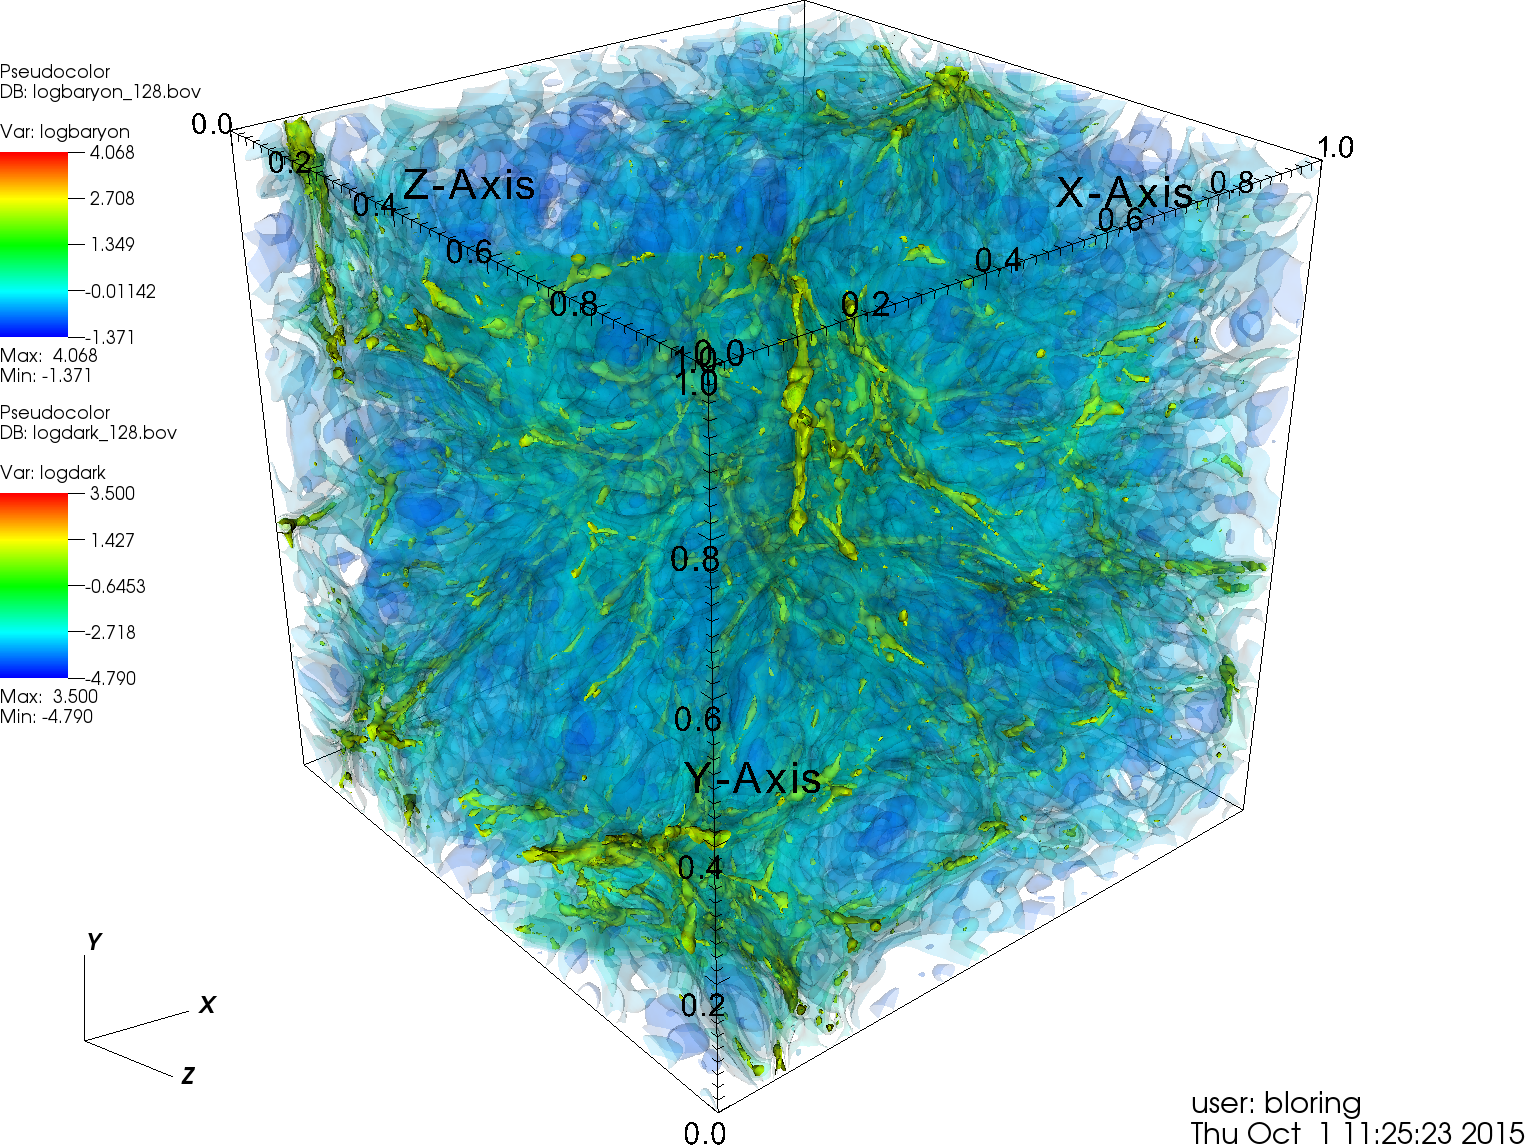
\includegraphics[height=3.0in]{./cosmology_test_case_0080.png}
 % cosmology_test_case_0080.png: 1703x1220 pixel, 300dpi, 14.42x10.33 cm, bb=0 0 409 293
 \caption{$256^3$ cosmology dataset}
 \label{fig:cosmo_data}
\end{figure}
This is a $256^3$ cosmology dataset. I took 10 iso-surfaces of one field and made them 16\% opaque, and took one iso-surface of another field and made it 100\% opaque. It exercises both rendering passes. there is quite a bit more geometry in the transparent pass. I really wanted to exercise the ordered compositing. My benchmarks used a resolution of 1700x1220, which is how I normally run visit.


opaque: 1
The actual number of zones is 488520.
transparent: 10
The actual number of zones is 9884369.

\subsection{Plasma}
\begin{figure}[ht]
 \centering
 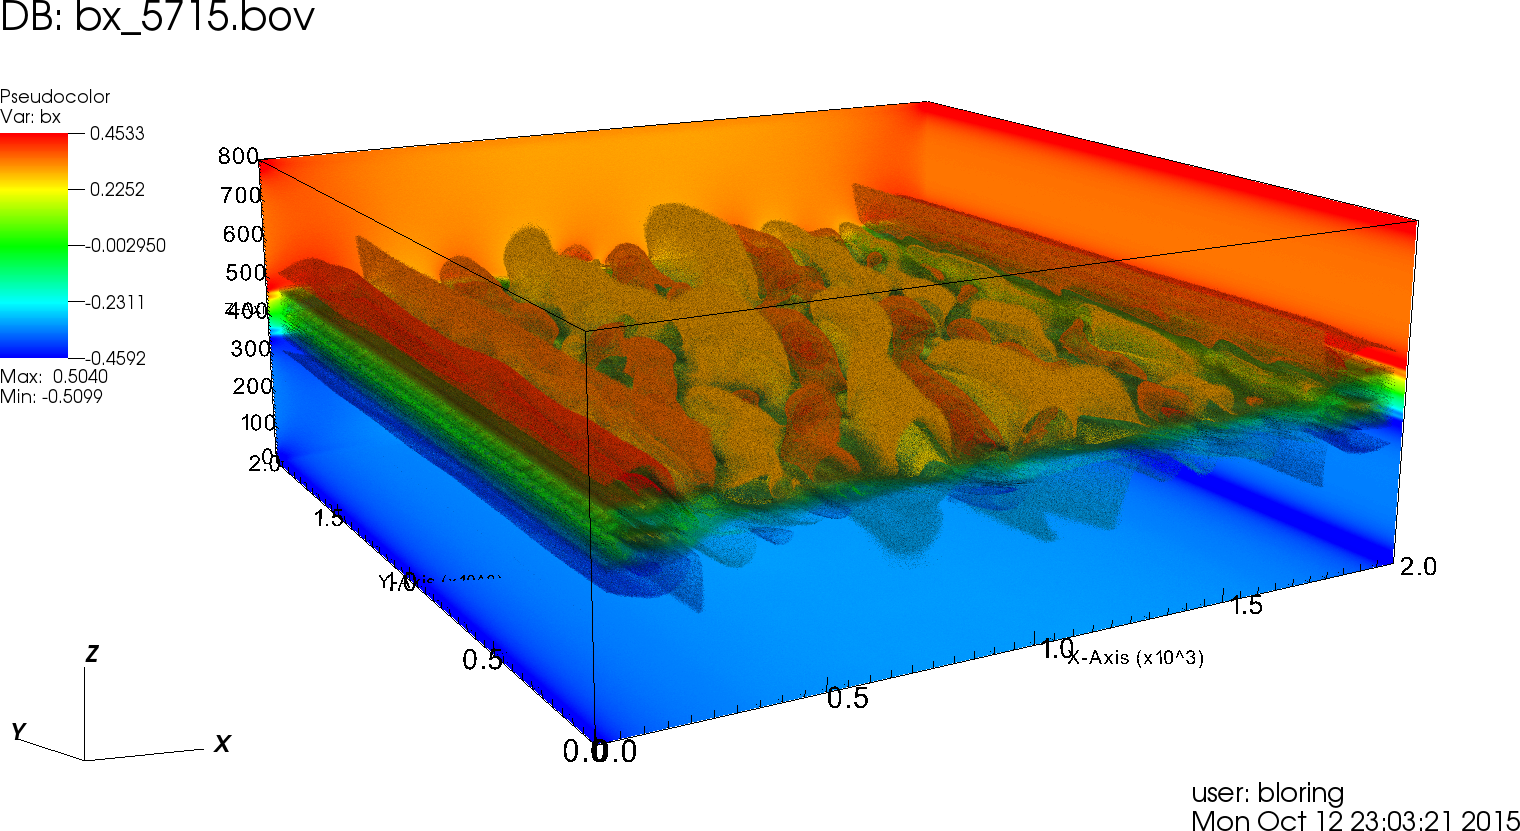
\includegraphics[height=3.0in]{./vpic_test_case_0030.png}
 % vpic_test_case_0030.png: 1703x1220 pixel, 300dpi, 14.42x10.33 cm, bb=0 0 409 293
 \caption{$2000^2 \times 800$ plasma dataset}
 \label{fig:vpic_data}
\end{figure}

slices:
The actual number of zones is 3996001.
The actual number of zones is 1597201.
The actual number of zones is 1597201.
iso surfaces: 20
The actual number of zones is 464815961.


\section{Results}
 \begin{figure}
 \centering
 \begin{minipage}[c]{0.5\textwidth}
 \begin{center}
 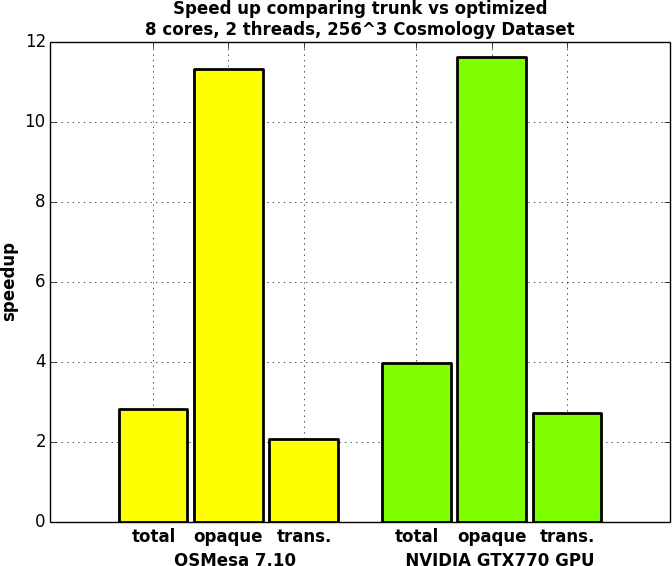
\includegraphics[height=2.25in]{./speed_up_cosmo.png}
 \end{center}
 \end{minipage}
 \begin{minipage}{0.3\textwidth}
 \begin{center}
 \def\arraystretch{1.5}
{\footnotesize
\begin{tabular}{|c|c|c|}
 \hline
 \multicolumn{3}{|c|}{\bf{Speedup compared to trunk}} \\ \hline
\multirow{4}{*}{GTX770} & total & 3.58 \\ \cline{2-3}
 & opaque & 11.89 \\ \cline{2-3}
 & transparent & 2.34 \\ \hline
\multirow{3}{*}{OSMesa} & total & 2.83 \\ \cline{2-3}
 & opaque & 11.34 \\ \cline{2-3}
 & transparent & 2.08 \\ \hline
\end{tabular}} 
\end{center}
\end{minipage}
\caption{Speedup of total rendering and compositing time using 8 cores, and 2 threads, on the $256^3$ cosmology dataset. Total and per pass time are shown. In the opaque pass z-buffer compositng is used while in the transparent pass alpha blending is used. The GPU and OSMesa show a similar speed-ups.}
\label{fig:speedup_cosmo}
\end{figure}

 \begin{figure}
 \centering
 \begin{minipage}[c]{0.5\textwidth}
 \begin{center}
 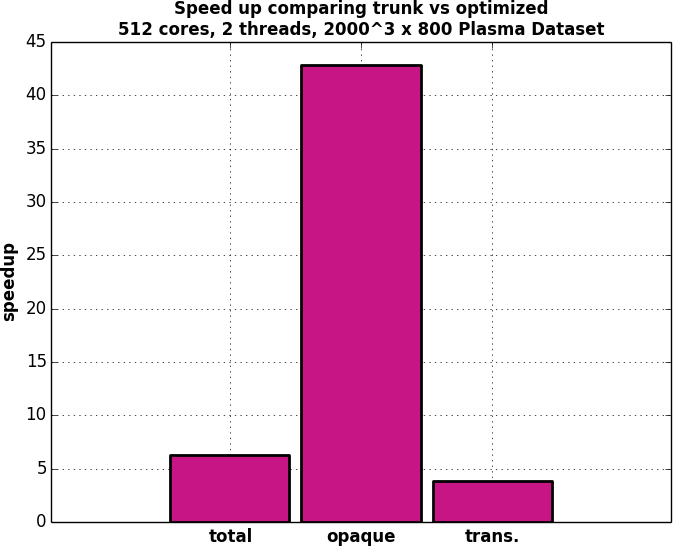
\includegraphics[height=2.25in]{./speed_up_vpic.png} 
 \end{center}
 \end{minipage}
 \begin{minipage}{0.3\textwidth}
  \begin{center}
  \def\arraystretch{1.5}
{\footnotesize
\begin{tabular}{|c|c|c|}
 \hline
 \multicolumn{3}{|c|}{\bf{Speedup compared to trunk}} \\ \hline
\multirow{3}{*}{OSMesa} & total & 6.31 \\ \cline{2-3}
 & opaque & 42.85 \\ \cline{2-3}
 & transparent & 3.82 \\ \hline
\end{tabular}}
\end{center}
\end{minipage}
\caption{Speedup of rendering and compositing using 512 cores, and 2 threads, on the $2000^2 \times 800$ plasma dataset. Total and per pass time are shown. In the opaque pass z-buffer compositng is used while in the transparent pass alpha blending is used. For both opaque and transparent passes the speed up has grown compared to the 8-core tests. The opaque pass we acheived over 40 times speedup.}
\label{fig:speedup_vpic}
\end{figure}








Here is the comparison of the total render and composite time. red bars show times using the trunk and blue bars show times using my patch.

Here is the same but just the opaque pass. The opaque pass benefits substantially from the optimization. I included this one because it shows general the impact of my optimization. The speed up is not just from the ordered compositing, which only comes into play in the transparent pass.


Here is the same but just the transparent pass.


\subsection{Ordered Compositing}
I implemented ordered compositing in VisIt. It works with both VisIt's native compositer, and IceT. It detects when order compositing can be used and switches itself on automatically. There's also a GUI option to disable it. It is on by default. Here is the speed up of ordered compositing vs VisIt's distributed geometry sort. Ordered compositing is more than 2x faster. This is only 8 cores and a relatively small dataset. I will also document it on larger data on Cori or Edison, but I predict that the gap will only get wider as it scales up.

\subsection{Depth Peeling}
\begin{figure}
\centering
\begin{minipage}{0.28\textwidth}
\begin{center}
 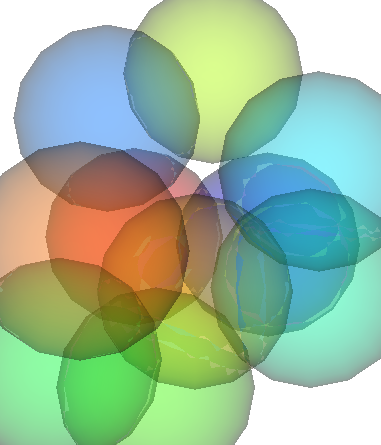
\includegraphics[height=2.0in]{./spheres_with_sort_crop.png}
 \end{center}
\end{minipage}
\begin{minipage}{0.28\textwidth}
 \begin{center}
 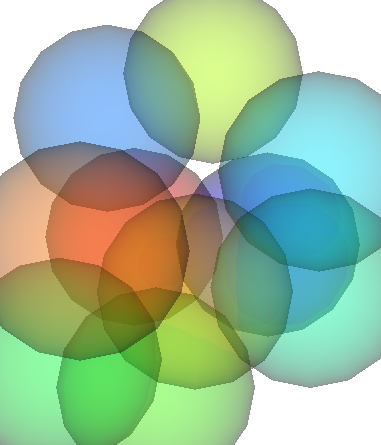
\includegraphics[height=2.0in]{./spheres_with_depth_peel_crop.png}
\end{center}
\end{minipage}
\begin{minipage}{0.3\textwidth}
 \begin{center}
 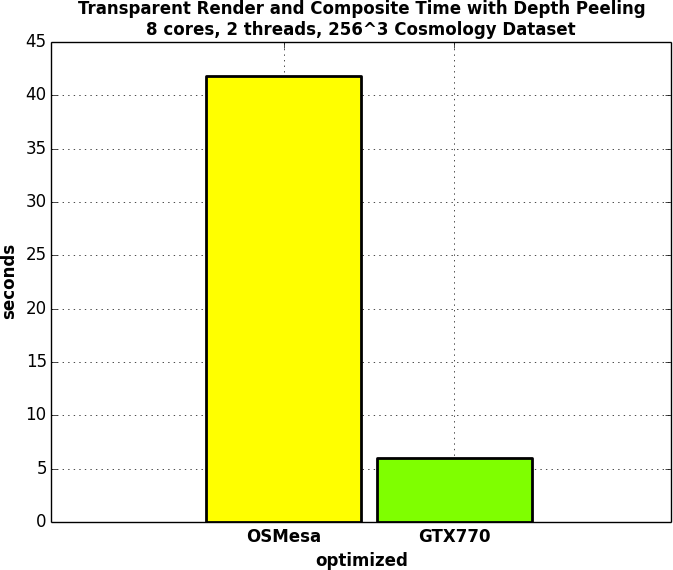
\includegraphics[height=2.25in]{./depth_peeling_time_cosmo.png}
\end{center}
\end{minipage}
\caption{depth peeling}
\label{fig:speedup_vpic}
\end{figure}
I investigated the use of depth peeling. The conclusion is that it is very slow compared to geometry sort. Here is the time from the transparent pass rendering the $256^3$ cosmology dataset. In my test it took 40 seconds on OSMesa, and as a result is unusable here. It took 6 seconds on my GTX480, still way too slow. But this is a complex scene and it takes quite a few peels. For simple scenes I found that it is slower than the local geometry sort but can be fast enough not to be a problem. I added a GUI option to enable it. It's is off by default.


Despite its poor performance depth peeling is a useful feature  because VisIt doesn't split intersecting geometry. This shows a comparison of rendering using local geometry sort on the left and depth peeling on the right. You can see artifacts in the geometry sort because VisIt doesn't handle intersecting geometry. Depth peeling is slower but produces the correct result.

  


\section{VisIt integration:}
Here are the GUI elements that control the new features. The default settings are shown.










The patch is now quite large and while I have tested it extensively, there may be some issues that I didn't find. I plan to run it through VisIt's regression suite and pick off any issues I can identify. I'd like to commit it after. Let me know if you have any comments


\end{document}
